\documentclass[12pt]{article}
\usepackage[top=1in, bottom=1in, left=1in, right=1in]{geometry}

\usepackage{setspace}
\onehalfspacing

\usepackage{amssymb}
%% The amsthm package provides extended theorem environments
\usepackage{amsthm}
\usepackage{epsfig}
\usepackage{times}
\renewcommand{\ttdefault}{cmtt}
\usepackage{amsmath}
\usepackage{graphicx} % for graphics files
\usepackage{tabu}

% Draw figures yourself
\usepackage{tikz} 

% writing elements
\usepackage{mhchem}

% The float package HAS to load before hyperref
\usepackage{float} % for psuedocode formatting
\usepackage{xspace}

% from Denovo Methods Manual
\usepackage{mathrsfs}
\usepackage[mathcal]{euscript}
\usepackage{color}
\usepackage{array}

\usepackage[pdftex]{hyperref}
\usepackage[parfill]{parskip}

% math syntax
\newcommand{\nth}{n\ensuremath{^{\text{th}}} }
\newcommand{\ve}[1]{\ensuremath{\mathbf{#1}}}
\newcommand{\Macro}{\ensuremath{\Sigma}}
\newcommand{\rvec}{\ensuremath{\vec{r}}}
\newcommand{\vecr}{\ensuremath{\vec{r}}}
\newcommand{\omvec}{\ensuremath{\hat{\Omega}}}
\newcommand{\vOmega}{\ensuremath{\hat{\Omega}}}
\newcommand{\sigs}{\ensuremath{\Sigma_s(\rvec,E'\rightarrow E,\omvec'\rightarrow\omvec)}}
\newcommand{\el}{\ensuremath{\ell}}
\newcommand{\sigso}{\ensuremath{\Sigma_{s,0}}}
\newcommand{\sigsi}{\ensuremath{\Sigma_{s,1}}}
%---------------------------------------------------------------------------
%---------------------------------------------------------------------------
\begin{document}
\begin{center}
{\bf NE 250, F15\\
October 21, 2015 
}
\end{center}

\textbf{Monte Carlo} for neutral particle transport

So far we've talked about the diffusion equation, derived the transport equation a few ways, and talked about the adjoint. \\
I'd like to spend the next bit of time talking about Monte Carlo methods, variance reduction, and how we can use the adjoint with variance reduction (note that I've totally just canned the syllabus). \\
After that we'll move into discretization and solution methods for the deterministic transport equation. 

What is Monte Carlo?
  \begin{itemize}
  \item The use of \textit{random processes} to determine a \textit{statistically-expected} solution to a problem
  \item Random processes can fulfill two roles:
  \begin{itemize}
    \item Statistical approximation to \textit{mathematical equations}
    \item Statistical approximations to \textit{physical processes}
  \end{itemize}   
  \item Construct a random process for a problem, 
  \item Carry out a numerical simulation by N-fold sampling from a (pseudo-)random \# sequence
\end{itemize}

For MC in radiation transport, we simulate many independent particles in a system:
\begin{itemize}
\item Treat each physical process as a \textit{probabilistic process}
\item \textit{Randomly sample} each process using an independent stream of pseudo-random numbers
\item Follow each particle from birth until it no longer matters
\item Accumulate the contributions of each particle to find the statistically-expected mean behavior and variance
\end{itemize}

\begin{figure}[h!]
\begin{center}
  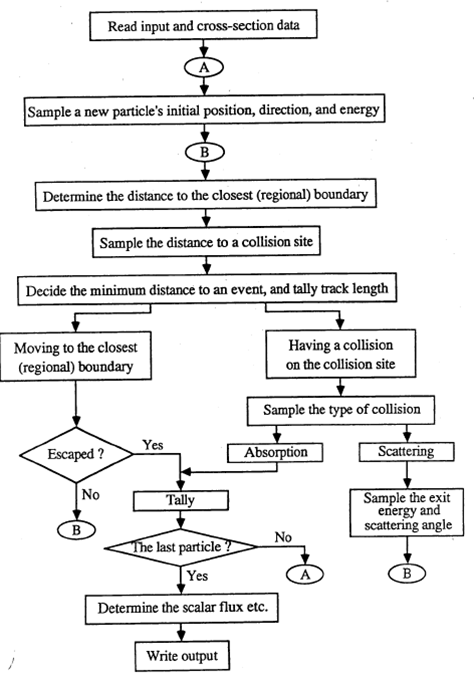
\includegraphics[height=6 in,clip]{../figs/MC-algorithm}
\end{center}
  \caption{Monte Carlo neutral particle transport algorithm}
  \label{fig:mc-algo}
\end{figure}

\textbf{WHY} use Monte Carlo?\\
Monte Carlo, when done properly, can be highly accurate and can be considered a ``gold standard" answer. Table~\ref{tab:comparison} compares MC and deterministic methods.
%
\begin{table}[h!]
\begin{center}
\begin{tabu}{| X | X |}
\hline
Monte Carlo         & Deterministic \\\hline
% -----------------------
* General geometry    & * Discretized geometry \\
* Continuous Energy   & * Multigroup in energy\\
* Continuous in Angle & * Angular Quadrature\\
* Number of particles governs solution accuracy & * Discretization and solver methods govern solution accuracy \\
* Must adequately sample phase space & * Must adequately discretize phase space \\
* Solutions have statistical error & * Solution contains truncation error\\
* \textbf{Local} solutions only; variable quality & * \textbf{Global} solutions; equal quality \\\hline
% -----------------------
* Easy to parallelize on CPUs & * Can be complicated to parallelize on CPUs\\
* Slow & * Can be quite fast \\
* Might be memory intensive & * Might be memory intensive \\
* Need efficient Variance Reduction & * Need acceleration methods \\\hline
  \end{tabu}
  \caption{Comparison of Monte Carlo and Deterministic Methods}
  \label{tab:comparison}
\end{center}
\end{table}
%
Figure~\ref{fig:mc-algo} shows the algorithm that is basically what happens in MC. \\
We will go through the very basics of the ideas about probability distributions, sampling, scoring, and statistics.

%-------------------------------------------------------
-------------------------------------------------------\\
\textbf{Probability Distributions}\\
We need to figure out all of these things about how particles are moving around in our system, but how do we do it?\\
We get functional expressions of the probability that various things will happen and try to take enough samples to effectively capture those expressions.
%
\begin{itemize}
\item For a random variable, $x$, the probability that $x$ will have a value between $a$ and $b$ is $P\{a \leq x \leq b\}$.
%
\item The \textit{probability density fuction} expresses the likelihood that $x'$ will take on a value between $x$ and $x+\Delta x$:
\begin{align*}
\lim_{\Delta x \to 0} f(x)\Delta x &= P \{ x \leq x' \leq x + \Delta x \}\\
\int_a^b f(x) dx &= P\{a \leq x \leq b\}
\end{align*}
%
\item We often normalize this PDF to integrate to one, using one of
\begin{equation}
\int_{-\infty}^{\infty} f(x) dx = 1 \quad \text{or} \quad
\int_{x^-}^{x^+} f(x) dx = 1 \nonumber
\end{equation}
%
\item To get the probability that our random variable $x'$ is less than or equal to some value $x$, we use a \textit{cumulative distribution function}:
\begin{align*}
F(x) &= P\{x' \leq x\} \\
F(x) &= \int_{-\infty}^{x} f(x') dx' \\
\lim_{x \to \infty} F(x) &\equiv F(\infty) = 1 \\
\lim_{x \to -\infty} F(x) &\equiv F(-\infty) = 0 \\
P \{ a \leq x' \leq b \} &= F(b) - F(a)
\end{align*}
\end{itemize}

Various physical phenomena can be represented by probability distributions
\begin{itemize}
  \item Photon emission energy: Each possible energy has a different probability (intensity)
  \item Scattering cross-sections: Each possible scattering angle has a different probability as a function of the energy
  \item Transmission through a medium: Probability of reaching a particular position
depends on the cross-section
\end{itemize}
%
We in one way or another get these PDFs and/or CDFs and use random numbers to select values for use in simulation.


\end{document}
